\chapter{Summary(Discussion, Conclusion, and Future Work)}

The results obtained from the procedure of cross-validation indicate that there is an almost negligible difference between the mean of the errors when comparing all the different training sizes. This result is the same for both models with and without the added underplating of \cite{Mariani2013} with variations in both being around 0.1km. This means that for this model the size of the testing set does not matter because all sizes above 2/3 of the data will arrive at the same conclusion. It is worth noting though that the model with the intrusion implemented has on average higher RMS values than that without the intrusion, this was initially expected. The residual values between the model and the point estimates show that the error on the whole model was around 2.3-2.6km but this likely varies from region to region. However, this is a viable method to estimate Moho model errors using cross-validation that can be extended past just South America and to different parts of the Earth given that there are seismic point estimates to carry out the method of repeated random sub-sample validation.
\section{Modelling a subducting slab to combat uncertainty}
Even though the method was successful in estimating the error on the model this RMS error value only gives one singular uncertainty on the model, this can be skewed by few large disparities between the model and the point estimates. This is very much so the case, in the Andes due to the active plate tectonics in the area leading to a sharp increase in Moho depth when compared to the surrounding depths, something which cannot be modelled properly due to the regularization parameter which keeps the model smooth and without sharp vertical variations over short distances. Given that the regularization parameter was selected through hold-out cross-validation, it is not plausible to change this value as it can cause instability in other parts of the model, where Moho depths are estimated well when compared to previous results. One solution that \cite{Uieda2016} suggested was to implement a separate smoothness regularization for areas in South America such as the Andes or not to have one for these regions at all. Another solution to this problem that may be easier to implement into the code would be to model the subducting Nazca plate using a Slab2 model from rockhound \citep{uieda_leonardo_2020_3627166}. The only issue with this is that in the model the crust and lithosphere thickness and density would have to be assumed and then these can be mapped onto tesseroids. This procedure will address the shallow Moho under the Andes and the surrounding area and should in theory decrease the MSE values obtained from the repeated random sub-sample validation. On top of this, it would be straightforward to see how much this method would improve the error estimates on the model by comparing the difference between identically derived models with the only change being one notebook including the Slab2 model and the other not. With the deep Moho values (upwards of 40km) being underestimated in South America for many models \citep{vanderMeijde2013} \citep{Reguzzoni2015}. One way to obtain better MSE values would be to change the location of the model to an area that lacks significant tectonic activity, for example, Africa. Although, no region is free from tectonic movement and the East African Rift Zone is the most prominent tectonic regime here. Despite this, the Moho depths in this region do not surpass 50km, and so this is a viable choice. However, if using the same procedure of cross-validation here, Africa would present the same problems as South America with the locations and clustering of seismic point data around the coast of the continent. This issue like that of South America would be due to the environment in central Africa along with financial hardship as seismic surveys are expensive to carry out. Although overall the RMS values or errors on the model should be lower as the model can be fit better to the seismic point estimates through regularization keeping the Moho surface smooth.
Even if the focus was turned back to South America the CRUST1.0 model used \citep{Laske2013} doesn't consider and model the subducting slab either, though taking this into account the final Moho depth model produced using the code from \cite{Uieda2016} has discrepancies with the CRUST1.0 model. The main reason for this is that CRUST1.0 uses seismic point estimates and extrapolates them for regions where no data is present and South America this most notably is the Amazon Rainforest. On the other hand, the Uieda model is computed using gravitational data, rather than seismic. One area where these models somewhat disagree is in the Andes and to the east of the vast mountain range. The CRUST model predicts a deeper Moho through extrapolation due to the isostatic balancing from the Andes whereas this part is modelled to be much shallower in \cite{Uieda2016} as there is gravity data for the foreland basins.
\section{Blocked testing sets}
The procedure used in this study as mentioned used repeated random sub-sample validation to estimate the errors on the model as a result the singular error value attained is the average error on the whole model across the continent of South America. When this is taken into account as a large-scale representation, there is a lack of information given as the areas of larger and smaller disparity are not known. Rather than using "random" sampling of the data to separate it into the training and testing set instead the data can be split up using a method of "Blocking". By selecting points for the testing set by geographical area rather than randomly an uncertainty estimate can be calculated for just the region that the seismic point estimates span. By using this method the likely larger errors seen in the Andes can be separated from the areas of the continent where the model and the point estimates agree very well with each other leading to smaller RMS values in blocked areas with small disparities. However, "Blocking" with limited seismic estimates in some regions and large quantities of these estimates grouped in tight clusters may lead to different validating sizes, which as seen in the results is not much of a problem as the 3 different sizes used achieved very similar mean RMS values. For this method to work the blocked regions must be of equal or similar size as a testing size of 100 points cannot be compared to a section with only 10 seismic point estimates. So when implementing "Blocking" for South America areas where there are a large proportion of seismic points such as the Andes may have to be split into two or more regions. However, rather than gaining an error estimate for the model for the Andes or another high cluster region as a whole there would be multiple error values attained and would account as a separate RMS value per region. This uneven cluster would lead to errors for regions of possibly vastly different sizes depending on the testing size collected, with the smaller the subset the more areas there are and likely the more computationally expensive the process will be.
\section{Degrees of freedom in density estimations}
The code implemented by \cite{Uieda2016} uses cross-validation to estimate the best model hyperparameters before producing the final model. Overall, the misfit between the point estimates and the model is small, but in some places, the model has large disparities with the seismic point estimates. This is partially due to the singular density contrast used across the whole continent for the model. South America is a tectonically active region and will have geological units vastly ranging in densities from the less dense sedimentary rocks and basins to the very dense igneous intrusions. So one way of accounting for this is adding in more degrees of freedom in density estimations. This method has been implemented in \cite{Haas2020} using seismic regionalization that splits up the continent of South America into 6 different density contrasts (see Figure~\ref{fig:haas}).
\begin{figure}[h]
  \begin{center}
    % Width can be set to particular size (10cm) or relative to the page size,
    % like 0.5\textwidth (for half page) or \textwidth (for full page).
    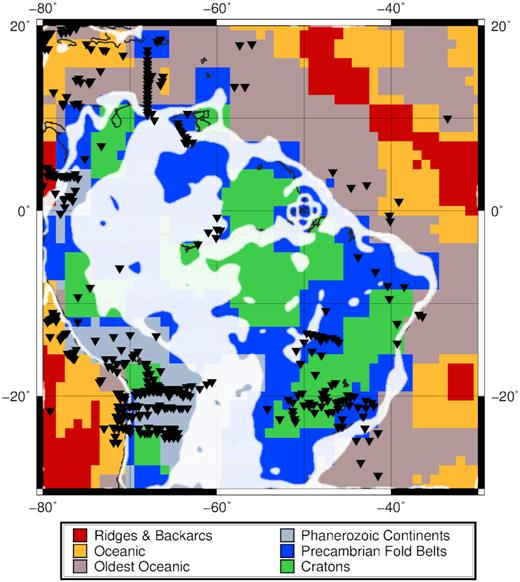
\includegraphics[width=0.5\textwidth]{figures/Haas-blocking}
  \end{center}
  \caption{
   Geologic units from seismic regionalization superimposed with estimated Moho depth of between 28km to 32km. The black triangles represent seismic stations. After \cite{Haas2020}.
  }
  % Label used to reference the figure in the text.
  \label{fig:haas}
\end{figure}
These density values are attained by using surface-wave tomographic models seen in \cite{Schaeffer2015global}. If this method were implemented into this code then it is likely that the mean errors between the model and the seismic constraints would decrease as the model created through inversion will better fit the seismic points whilst still having a smooth solution through a regularization coefficient. 
However, the main issue that arises is that the model requires the user to manually choose how many different regions there will be. For every extra region added to the model there will be an exponential increase in the computational time, and after a certain number of different density contrasts adding more will not improve the model. Hence a trade-off is needed between the number of regions and the computational time. In \cite{Haas2020} as mentioned 6 regions with different density contrasts were used and comparing this model to \cite{Uieda2016} the frequency of residuals is clustered more towards smaller values whereas the latter model has a slightly higher representation when it comes to larger residual Moho depths (see Figure~\ref{fig:Haas_Uieda}).
\begin{figure}[h]
  \begin{center}
    % Width can be set to particular size (10cm) or relative to the page size,
    % like 0.5\textwidth (for half page) or \textwidth (for full page).
    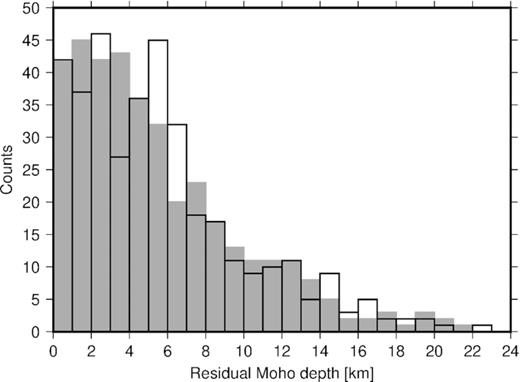
\includegraphics[width=0.5\textwidth]{figures/Haas-Uieda}
  \end{center}
  \caption{
   Histogram comparing \cite{Haas2020} (grey bars) residual Moho depths to \cite{Uieda2016} model (black bars). The bin size for each model is 1km. From \cite{Haas2020}.
  }
  % Label used to reference the figure in the text.
  \label{fig:Haas_Uieda}
\end{figure}
A possible future avenue could be to put the computational time aside and see how many different density regions can be implemented into the code until adding more in does not decrease the mean size of the Moho residuals between the model and point estimates.